\chapter{软件分布式共享内存系统与RDMA技术介绍}\label{chap:sdsm}{
    本文研究的基础主要包括软件分布式共享内存系统的实现和远程直接内存访问(RDMA)技术两个方面,本章将分别对这两项技术进行系统性阐述。
    针对软件分布式共享内存系统,将介绍其关键技术,即内存一致性以及系统的实现层次;
    针对 RDMA 技术,将主要介绍其通信原理、RDMA 实现与相关通信库以RDMA通信编程方面的内容。

    \section{软件分布式共享内存关键技术}\label{软件分布式共享内存关键技术}

    \subsection{实现层次}\label{sec:implementations}
    软件 DSM 系统实现方式灵活,可以在系统软件(操作系统或编译器)、运行时库、语言等层次上实现。
    \begin{itemize}
        \item \textbf{基于操作系统修改的软件DSM系统}:
              早期的软件 DSM 系统如 IVY\citep{likai1988ivy} ,Munin\citep{bennett1990munin}等通过依赖或修改系统软件来实现共享虚拟内存抽象和一致性管理。
              以 IVY 为例, IVY 会通过修改操作系统中的内存管理模块(Memory Management Unit, MMU)来监测远程访问,当处理机访问非本地页时,将触发缺页中断,并由 MMU 向远端取页;
              这种方案由于需要系统软件支持会导致可移植性差。

        \item \textbf{基于用户库形式软件 DSM 系统}:
              以用户库形式提供给开发者的全软件 DSM 系统是更为常见的实现。
              通过操作系统接口检测缺页异常并处理。系统初始化时使用 mmap() 建立共享虚拟内存与本地内存的映射,并通过 mprotect() 修改共享页权限。
              当访问远端节点的共享页时,会发生越权访问,操作系统产生段违例信号(SIGSEGV),由预先注册的信号处理程序捕获并完成远程取数和权限授予。
              此类方案完全在用户空间运行,无需修改硬件或系统软件,可移植性强,TreadMarks、CRL、OpenSHMEM、JIAJIA等均采用此种实现方式。

        \item \textbf{基于语言或语言扩展级别的 DSM 系统}:
              语言或语言扩展级别的 DSM 系统在高性能计算社区发展为分区全局地址空间(PGAS)语言,通过扩展现有语言规范提供分布式共享内存编程模型,
              适合 Exascale 规模高性能并行计算。典型代表包括面向 Fortran 的 Coarray Fortran~\citep{numrich1998coarrayfortran, coarryfortran2}、
              面向 Java 的 Titanium~\citep{Yelick1998Titanium}、
              面向 C 的 UPC~\citep{bonachea2013UPC}(Unified Parallel C)以及面向 C++ 的 UPC++~\citep{bachan2019upc++}。
              与传统 DSM 系统的区别在于显式远程数据访问,程序员需明确指定数据来源。实现上依赖编译器和通信中间件层(如 GASNet~\citep{Bonachea2018GASNetEX})支持。
    \end{itemize}

    % \begin{figure}
    %     \centering
    %     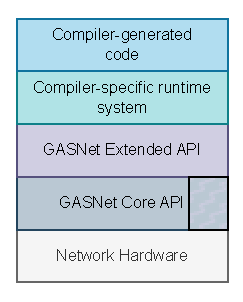
\includegraphics[width=0.3\textwidth]{Img/GASNet.drawio.pdf}
    %     \bicaption{\enspace GASNet 层系统图}{\enspace GASNet layer disgram}
    %     \label{fig:GASNET}
    % \end{figure}

    % \subsection{通信机制}
    % 软件 DSM 系统依赖底层的消息传递机制来实现上层的虚拟共享抽象。不同网络环境和协议实现的消息传递机制在通信流程和开销上展现出显著差异。

    % \begin{enumerate}
    %     \item 为了追求更高的性能和可扩展性,传统 DSM 系统通常更倾向于采用低延迟的 UDP。
    %           在此基础上,可以分为由SIGIO信号驱动的单线程模型,和采用划分通信任务的多线程模型;
    %     \item RDMA 网络为现代软件 DSM 系统通信提供性能优势。在UDP的基础上,高带宽、低延迟的特性极大的降低了通信传输延迟;
    % \end{enumerate}

    \subsection{内存一致性模型}
    内存一致性模型限制了系统可以执行内存访问的顺序。维护内存一致性是软件 DSM 系统的关键问题,核心在于何时以及如何传播对共享内存的更新。

    \begin{itemize}
        \item \textbf{严格一致性模型(Strict Consistency):} 严格一致性模型要求任何一次读操作总是返回最近一次对相同对象的写入结果,实现需要全局时钟同步和零通信延迟的理想条件。

        \item \textbf{顺序一致性(Sequential Consistency):} 顺序一致性是最直观的内存一致性模型,最早由 Lamport 形式化定义,要求系统中所有进程对共享数据的操作必须呈现出一个全局的顺序,同时每个进程内部的操作顺序必须与程序中给定的顺序保持一致。

        \item \textbf{处理器一致性(Processor Consistency):} 处理器一致性比顺序一致性弱,核心特性可以概括为以下两条规则:
              \begin{enumerate}[label=\arabic*.]
                  \item 每个处理器内部发出的所有写操作必须以程序中的顺序被其他处理器观察到。
                  \item 对于同一内存地址,所有处理器都必须看到相同的写顺序;对于不同地址的写操作,各处理器可以看到的顺序不完全一致。
              \end{enumerate}

        \item \textbf{弱一致性(Weak Consistecny):} 弱一致性模型的核心机制在于区分同步操作与普通访存操作,
              开发者通过显式的同步操作保护共享内存的写入,确保多个处理器对同一共享单元的写操作互斥,
              适用于对性能要求较高且数据一致性可容忍一定延迟更新的场景。

              \begin{figure}[!htbp]
                  \centering
                  \begin{subfigure}[b]{0.8\textwidth}
                      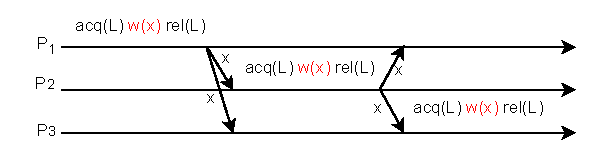
\includegraphics[width=\textwidth]{Img/急切更新释放一致性.drawio.pdf}
                      \caption{急切更新释放一致性}
                      \label{fig:eager-release-consistency}
                  \end{subfigure}
                  \\
                  \begin{subfigure}[b]{0.8\textwidth}
                      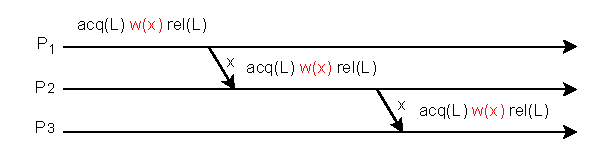
\includegraphics[width=\textwidth]{Img/懒惰更新释放一致性.drawio.pdf}
                      \caption{懒惰更新释放一致性}
                      \label{fig:lazy-release-consistency}
                  \end{subfigure}

                  \bicaption{\enspace 急切更新释放一致性 vs 懒惰更新释放一致性}{\enspace Eager release consistency vs Lazy release consistency}
                  \label{fig:oaspl}
              \end{figure}

        \item \textbf{急切更新释放一致性(Release Consistency):} 释放一致性的核心思想是把弱一致性中的同步操作进一步划分为获取操作(acquire)和释放操作(release)。只在特定的释放操作时才传播对共享内存的更新以保证数据一致性,而不是在每次访问共享内存时都强制同步。

        \item \textbf{懒惰更新释放一致性(Lazy release Consistency):} 懒惰更新释放一致性将更新传播的目的地范围限制为下一个获取锁的节点。这进一步减少了系统中通信消息的数量。
              图~\ref{fig:oaspl}说明懒惰更新释放一致性与急切释放一致性的通信比较。

        \item \textbf{域一致性(Scope Consistency):} 域一致性引入了一致性域(consistency scope)的概念,可以简单地将一致性域视为由锁保护的临界区。
              通过这一概念隐式地建立起共享内存对象与同步对象之间的关联,进而限制每次传播的共享内存对象更新的范围,有效降低了通信数据量。

        \item \textbf{单项一致性(Entry Consistency):} 单项一致性最早由 Midway 系统提出。开发者需要显示建立共享变量与同步变量之间的关联,对每一个共享变量的访问都需要由关联的同步变量来保护。具体而言,当获取同步变量(acquire)时,仅传播与同步变量关联的共享变量的更新。
    \end{itemize}

    \section{RDMA 技术介绍}\label{RDMA 技术介绍}
    远程直接内存访问(Remote Direct Memory Access, RDMA)是一种广泛应用于高性能计算中的网络通信协议,它允许直接对远程内存进行读写操作,而无需依赖双方的操作系统或 CPU 的参与。
    如图~\ref{fig:DMA-RDMA}所示,RDMA 可视作直接内存访问(Direct Memory Access, DMA)在分布式系统上的扩展,把直接访问内存的范围从单机内存扩展到了远端内存。
    \begin{figure}[!htbp]
        \centering
        \begin{subfigure}[b]{0.50\textwidth}
            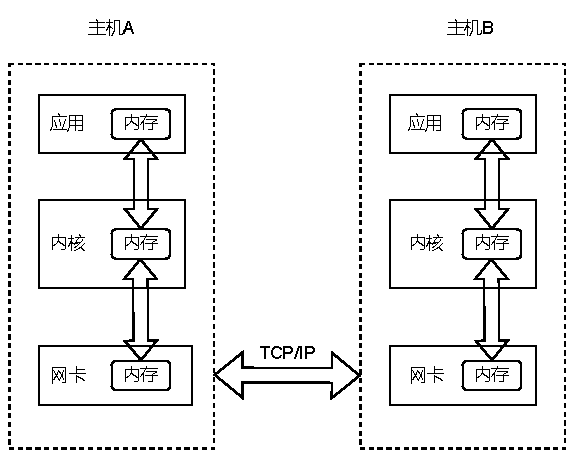
\includegraphics[width=\textwidth]{Img/TCP_IP通信.drawio.pdf}
            \caption{TCP/IP 通信}
            \label{fig:TCPIP}
        \end{subfigure}%
        ~~~~~% add desired spacing
        \begin{subfigure}[b]{0.50\textwidth}
            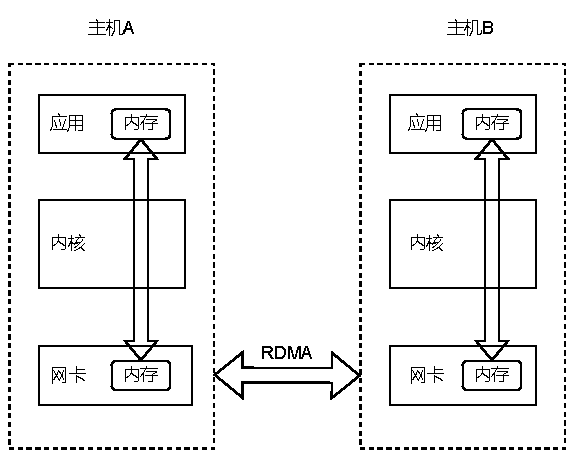
\includegraphics[width=\textwidth]{Img/RDMA通信.drawio.pdf}
            \caption{RDMA 通信}
            \label{fig:RDMA}
        \end{subfigure}
        \bicaption{\enspace DMA 与 RDMA 的比较}{\enspace Comparison of DMA and RDMA}
        \label{fig:DMA-RDMA}
    \end{figure}

    RDMA(Remote Direct Memory Access)是一种针对传统 TCP/IP 网络协议栈(图~\ref{fig:TCPIP})高延迟和高 CPU 开销问题的优化方案。
    在传统的 TCP/IP 通信模式下,跨机器的应用通信需要经历从用户到内核网卡的多个数据拷贝过程;
    相比之下,RDMA 通信模式(图~\ref{fig:RDMA})通过硬件直接访问内存,实现数据传输,无需拷贝至内核空间,
    同时由硬件完成协议处理并将数据传输至远端设备。

    RDMA 主要具备以下三大核心特性:
    \begin{enumerate}[label=\arabic*.]
        \item \textbf{零拷贝}(Zero-Copy)。数据可以直接从发送端用户空间传输到接收端用户空间,无需在内核空间与用户空间之间进行多次拷贝,从而减少延迟,提高吞吐量。
        \item \textbf{内核旁路}(Kernel Bypass)。RDMA 采用用户态驱动(如 Verbs API)直接控制网卡,绕过传统 TCP/IP 协议栈,避免内核态的数据封装、解析及中断处理,从而减少上下文切换的开销。
        \item \textbf{CPU 卸载}(CPU Offloading)。RDMA 网络协议处理完全由网卡硬件执行,
              且采用 RDMA 内存语义(如 RDMA Read/Write)进行数据传输时,远端 CPU 无需参与,从而降低了CPU 负担。
    \end{enumerate}

    \subsection{RDMA 通信模式与通信原语}

    \textbf{RDMA通信模式}

    RDMA 支持四种通信链路模式,分别是:
    可靠连接(RC)、不可靠连接(UC)、不可靠数据报(UD)、可靠数据报(RD)。这四种模式的通信特点如下:

    % \begin{figure}[!htbp]
    %     \centering
    %     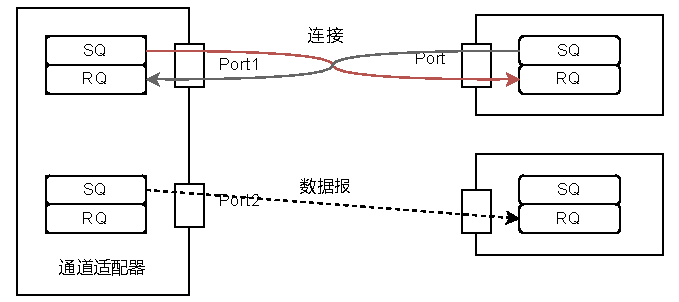
\includegraphics[width=\linewidth]{Img/RDMA队列对.drawio.pdf}
    %     \bicaption{\enspace RDMA 队列对}{\enspace RDMA Queue Pairs}
    %     \label{fig:rdma-queue-pairs}
    % \end{figure}

    \begin{itemize}
        \item \textbf{RC 模式}: RC 模式采用面向连接的方式,提供可靠且有序的传输服务。
              通信开始前,需要在通信双方的RC QPs之间建立私有连接。连接建立后,双方将以消息为基本单元进行通信。
              RC 模式具有可靠且有序的传输特性,且支持单向 Verbs 和原子操作,使其被广泛应用在对数据一致性、完整性和顺序性要求较高的场景中。
              例如,分布式存储系统 ~\citep{christopher2013pilaf, drago2014farm, xingda2020xstore}、
              高性能计算 ~\citep{graham2005OpenMPI, Huang2006MVAPICH2} 以及分布式事务系统 ~\citep{xingda2018DrTM+H} 等领域;
        \item \textbf{UC 模式}:UC 模式可视为 RC 模式的子集,面向连接但提供不可靠的传输服务(即不提供 Ack/Nak响应机制,不保证消息被对端成功接收),
              适用于对可靠性要求较低但对性能要求较高的场景,例如某些对实时性要求较高的视频应用;
        \item \textbf{RD 模式}:目前尚未有硬件支持 RD 模式,因此该模式尚未在实际应用中得到推广;
        \item \textbf{UD 模式}:UD 模式提供不可靠的数据报服务,无需建立连接,单个 QP 即可通过单播、多播或广播与其他 UD QPs 进行通信,
              但最大消息大小受 MTU 限制。适用于对可靠性要求较低或在应用层实现可靠性、规模较大且需要多播的应用场景~\citep{kalia2014herd,kalia2016fasst}。
    \end{itemize}

    \textbf{RDMA通信原语}

    RDMA 支持两类通信原语即所谓的动词(Verbs),双向动词和单向动词。

    \begin{itemize}
        \item \textbf{双向动词}: 双向动词又称为消息语义,包含 SEND 和 RECV ,适合传输控制消息,需要远端 CPU 参与提前下发接收请求,类似于传统的消息传递模型;
        \item \textbf{单向动词}: 单向动词又称为内存语义,包含 RDMA Read 、RDMA Write 和 RDMA 原子操作(Fetch-and-Add/FAA,Compare-and-Swap/CAS);
              RDMA 原子操作适合需要强一致性保证和低延迟并发控制的场景,RDMA Read 和 RDMA Write 可以绕过远端CPU,将大量数据直接读取或写入指定的内存位置。
    \end{itemize}

    表~\ref{tab:mode-verbs}展示了 RDMA 通信模式和通信原语的支持关系。

    \begin{table}[!htbp]
        \footnotesize% fontsize
        \setlength{\tabcolsep}{4pt}% column separation
        \renewcommand{\arraystretch}{1.5}% row space 
        \centering
        \begin{tabular}{lcccc}
            \hline
            %\multicolumn{num_of_cols_to_merge}{alignment}{contents} \\
            %\cline{i-j}% partial hline from column i to column j
               & Send/Recv  & RDMA Write & RDMA Read  & RDMA Atomic \\
            \hline
            RC & \checkmark & \checkmark & \checkmark & \checkmark  \\
            UC & \checkmark & \checkmark & \times     & \times      \\
            UD & \checkmark & \times     & \times     & \times      \\
            \hline
        \end{tabular}
        \bicaption{\enspace RDMA 通信模式与通信原语的关系}{\enspace Relation between RDMA communication mode and verbs}% caption
        \label{tab:mode-verbs}
    \end{table}

    \newpage
    \subsection{RDMA 通信流程}\label{sec:process}
    不同的 RDMA Verbs 在通信时有不同的执行的流程(大体流程及底层硬件流程见图~\ref{fig:rdma-Read}),以下是对几种常见 Verbs 通信流程的介绍。

    \begin{figure}[!htbp]
        \centering
        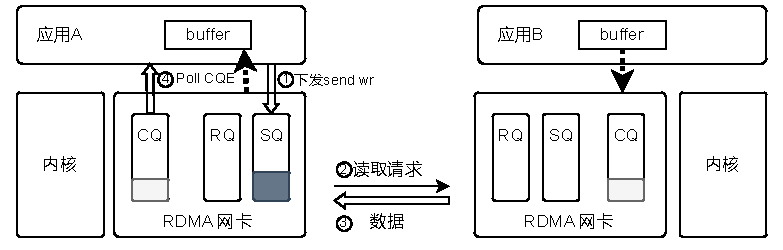
\includegraphics[width=\linewidth]{Img/RDMA-Read通信流程图.drawio.pdf}
        \bicaption{\enspace RDMA 通信流程图}{\enspace RDMA Read Communication Flow Diagram}
        \label{fig:rdma-Read}
    \end{figure}

    \begin{enumerate}[label=\arabic*.]

        \item \textbf{RDMA Read 通信流程}

              RDMA Read 用于直接读取远端内存。如~\ref{fig:rdma-Read}所示,其执行流程如下:
              \begin{enumerate}
                  \item 应用 A 向 SQ 中下发WQE,本地网卡根据 SQ 中的 WQE 向远端发送读取请求包。
                  \item 远端网卡接收到读取请求包后,根据包中携带的信息,读取应用 B 相应位置的内存,并发回数据。
                  \item 本地网卡接收到数据,根据 WQE 的信息将数据存入应用 A 的内存,并向 CQ 中存入CQE。
                  \item 应用通过轮询 CQ 获得 CQE,从中获取上一个请求的完成情况。
              \end{enumerate}

        \item \textbf{RDMA Write 通信流程}

              RDMA Write 用于直接写入远端内存,其执行流程如下:
              \begin{enumerate}
                  \item 应用 A 向 SQ 中下发WQE,本地网卡根据 SQ 中的 WQE 中的提示读取本地内存,组装数据包发往远端。
                  \item 远端网卡收到数据包后解析得到数据目的地址,将数据写入相应位置后返回 ACK 。
                  \item 本地网卡根据返回的 ACK 信息生成 CQE,并将其放入 CQ。
                  \item 应用通过轮询 CQ 获得 CQE,从中获取上一个请求的完成情况。
              \end{enumerate}

        \item \textbf{Send/Recv 通信流程}

              RDMA send recv负责两主机写作进行消息的发送与接收,其执行流程如下:
              \begin{enumerate}
                  \item 应用 B 向 RQ 下发接收工作请求,指定 RDMA 网卡接收数据的具体内存位置。
                  \item 应用 A 向 SQ 中下发发送工作请求,
                        本地网卡将根据 SQE 从应用 A 的内存取出数据并发往远端。
                  \item 远端 RDMA 网卡接收到数据后根据指定的位置将数据放入应用 B 的相应内存中。
                  \item 网卡将请求的执行状态放入 CQ 中,应用可通过轮询得到上一个请求的结果。
              \end{enumerate}

              从上述流程中可以看出,不同于Read/Write操作,Send/Recv 操作需要接收方 CPU 的参与。
    \end{enumerate}

    % 相比于RDMA Read, Send/Recv 和 RDMA Write 不需要网卡发回数据包,因此在传输小数据报时,
    % RDMA Write 和 Send/Recv 的传输延迟大约是 RDMA Read 的一半~\citep{kalia2014herd}(见图~\ref{fig:RDMA-Verbs-Latency})。
    % \begin{figure}[!htbp]
    %     \centering
    %     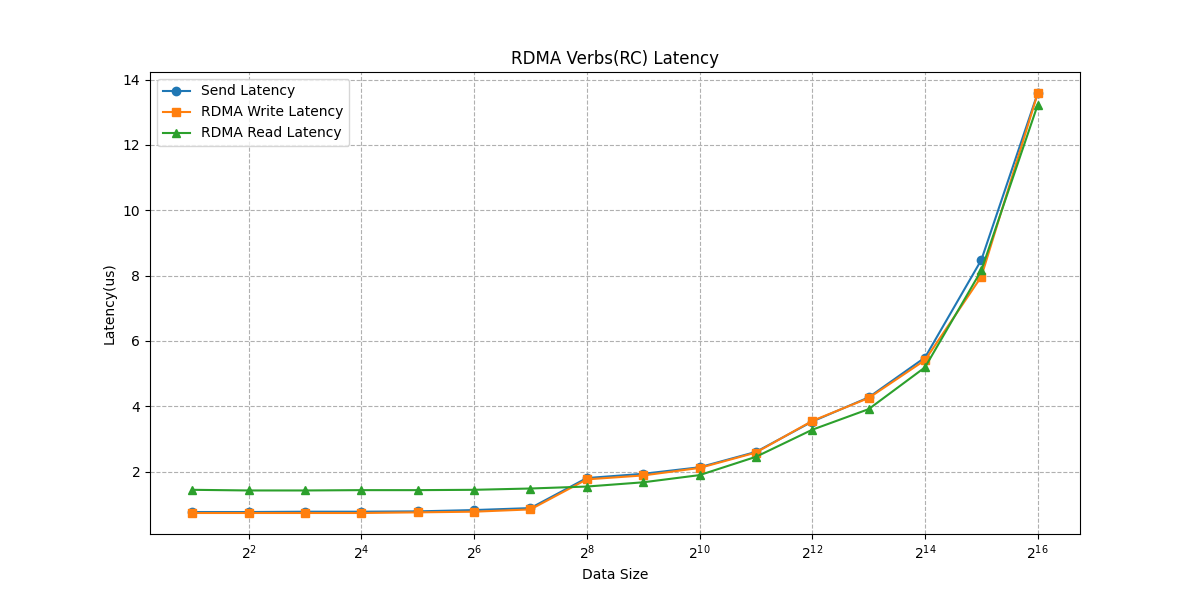
\includegraphics[width=\linewidth]{Img/verbs-latency.png}
    %     \bicaption{\enspace RDMA Verbs 通信延迟比较}{\enspace Comparison of Communication Latency of RDMA Verbs}
    %     {\small Note: 在Mellanox ConnectX-3 Pro 网卡可靠连接下的测试}
    %     \label{fig:RDMA-Verbs-Latency}
    % \end{figure}

    \subsection{RDMA 通信建连销毁流程}

    % 在传统通信模式中,主要有三种通信方式:
    % \begin{enumerate}
    %     \item 基于TCP协议的流式套接字(stream socket)
    %     \item 基于UDP协议的数据报套接字(datagram socket)
    %     \item 绕过传输层的原始套接字(raw socket)
    % \end{enumerate}

    % 见图~\ref{fig:Socket-Type}。
    % 在传统网络编程实践中,传输层协议的选择不仅决定socket的类型,还深刻影响整个通信子系统的设计,主要体现在连接管理、数据传输、错误处理等方面。
    % \begin{figure}[!htbp]
    %     \centering
    %     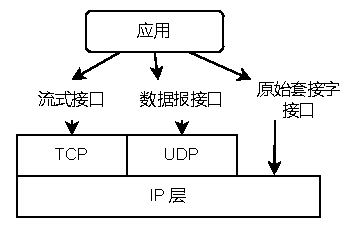
\includegraphics[width=0.35\linewidth]{Img/三种socket类型.drawio.pdf}
    %     \bicaption{\enspace 三种 Socket 类型}{\enspace The Three Socket Types}
    %     \label{fig:Socket-Type}
    % \end{figure}

    % 相比socket通信,RDMA 通信需要开发者深入了解底层网络协议与硬件特性。通信流程如下(以可靠连接为例):
    \begin{enumerate}[label=\textbf{步骤 \arabic*.}, leftmargin=0.5cm, align=left]
        \item \textbf{RDMA建立连接}
              \begin{itemize}
                  \item \texttt{ibv\_get\_device\_list()}, \texttt{ibv\_open\_device()}
                        选择指定设备并获取其上下文(ibv\_device);
                  \item \texttt{ibv\_alloc\_pd()},\texttt{ibv\_reg\_mr()} 创建保护域,注册内存区域(ibv\_mr);
                  \item \texttt{ibv\_create\_cq()},\texttt{ibv\_create\_qp()} 创建完成队列(ibv\_cq)与接收发送队列(QP)(ibv\_qp);
                  \item 采用传统Socket交换通信元数据,或直接采用 RDMA CM 建连。
              \end{itemize}

        \item \textbf{RDMA通信操作}

              详见第\ref{chap:sdsm}章的\ref{sec:process}小节。

        \item \textbf{资源回收操作}

              逆序销毁队列对、完成队列、内存区域等对象,释放保护域并关闭设备。
    \end{enumerate}

    \section{本章小结}

    本章 \ref{软件分布式共享内存关键技术} 节介绍了 软件分布式共享内存系统的实现层次,通信机制和内存一致性模型。

    本章 \ref{RDMA 技术介绍} 节介绍了 RDMA技术的基本原理和用法。
}